\documentclass{article}
\usepackage{v-test-paper}
% \usetikzlibrary{calc}

\usepackage{mathtools}


\usepackage[pages=some]{background}


\backgroundsetup{
  scale=1,
  color=black!90,
  opacity=1,
  angle=0,
  position=current page.south west,
  vshift=0,
  hshift=0,
  contents={
    \begin{tikzpicture}[remember picture, overlay]
      \fill[pattern=dots, pattern color=black!35] (current page.south west) rectangle (current page.north east);
    \end{tikzpicture}
  },
}

\title{\textsc{Compound Angles}}
\begin{document}
\maketitle


\begin{center}
    \begin{tikzpicture}
        [every node/.style={scale=0.85}]
        \def\radius{3.5}
        \def\angleA{20}
        \def\angleB{30}
        \tzcoor*(0, 0)(O){$O(0, 0)$}[bl]
        \tzcircle(O)(\radius)

        \tzaxes(0, 0)(1.5*\radius, 1.5*\radius){$x$}{$y$}
        
        \draw[->] (O)--(\angleB:\radius)coordinate(B) node [above right]{$B\left(\cos(B), \sin(B)\right)$};        
        \draw[->] (O)--(\angleA:\radius)coordinate(A) node[right]{$A\left(\cos(A), \sin(A)\right)$};
        \draw[->] (O)--(\angleA+\angleB:\radius) coordinate(C) node[above right]{$C\left(\cos(A+B), \sin(A+B)\right)$};

        \draw[->] (O)--(90-\angleA:\radius) coordinate(A') node[above right]{$A'\left(\sin(A), \cos(A)\right)$};

        \tzcoor*(0, \radius)(T){$T(0, 1)$}
        
       
        \tzanglemark[->](\radius,0)(O)(A){$A$}[pos=1.3](20pt)
        \tzanglemark[->](\radius, 0)(O)(B){$B$}[pos=1.2](35pt)
        \tzanglemark[->](\radius, 0)(O)(C){$A+B$}[pos=1.3](60pt)
        \tzanglemark[->](B)(O)(C){$A$}[pos=1.3](40pt)
        \tzanglemark[->](A')(O)(0, \radius){$A$}[pos=1.3](25pt)

        \draw[dashed] (A')--(B);
        \draw[dashed] (T)--(C);

    \end{tikzpicture}
\end{center}

\begin{align*}
    \intertext{Imagine standing at the center of a giant circle in the middle of a field. This circle represents the unit circle, with a radius of 1. Every point on the edge of this circle is exactly one unit away from you.}
    \intertext{First, you decide to walk along the edge of the circle to a point \(A\), which forms an angle \(A\) with the positive x-axis. At this point, you note down your coordinates: \((\cos A, \sin A)\). This is your first stop on the journey of discovering the sine addition formula.}
    \intertext{Next, you continue your walk to another point \(C\), which is at an additional angle \(B\) from point \(A\). So now, you are at angle \(A + B\) from the positive x-axis. You note down these coordinates as well: \((\cos(A + B), \sin(A + B))\).}
    \intertext{Nearby, there is a special point, \(T\), at the very top of the circle (the north pole if you will), with coordinates \((0, 1)\). Another interesting point is \(A'\), which is essentially point \(A\) but flipped over to \((\sin A, \cos A)\), aligning it vertically.}
\end{align*}


To unlock the secret of \(\sin(A + B)\), you imagine triangles forming between these points:
\begin{itemize}
    \item \textbf{Triangle OTC}: Formed by points \(O\) (the center), \(T\), and \(C\).
    \item \textbf{Triangle OBA'}: Formed by points \(O\), \(B\), and \(A'\).
\end{itemize}

\begin{align*}
    \intertext{You notice these triangles are congruent because they have two sides of the same length and the angle between them is the same. This means the distances from \(T\) to \(C\) and from \(B\) to \(A'\) are equal.}
    \intertext{You calculate these distances using the distance formula:}
    \text{Distance} &= \sqrt{(x_2 - x_1)^2 + (y_2 - y_1)^2} 
    \intertext{For \(TC\), the distance is:}
    &\sqrt{(0 - \cos(A + B))^2 + (1 - \sin(A + B))^2} 
    \intertext{For \(BA'\), the distance is:}
    &\sqrt{(\sin A - \cos B)^2 + (\cos A - \sin B)^2} 
    \intertext{Since these distances are equal:}
    \sqrt{\left(0-\cos\left(A+B\right)\right)^2 + \left(1-\sin\left(A+B\right)\right)^2} &= \sqrt{\left(\sin A - \cos B\right)^2 + \left(\cos A - \sin B\right)^2}\\
    \intertext{Squaring both sides,}
    \left(0-\cos\left(A+B\right)\right)^2 + \left(1-\sin\left(A+B\right)\right)^2 &= \left(\sin A - \cos B\right)^2 + \left(\cos A - \sin B\right)^2\\
    \cos^2\left(A+B\right) + 1 + \sin^2\left(A+B\right) - 2\sin\left(A+B\right) &= \sin^2 A - 2\sin A\cos B + \cos^2 B + \cos^2 A - 2\cos A\sin B + \sin^2 B\\
    1 - 2\sin\left(A+B\right) &= 1 - 2\sin A\cos B - 2\cos A\sin B\\
    \Aboxed{\sin\left(A+B\right) &= \sin A\cos B + \cos A\sin B}
\end{align*}

\begin{center}
    \textsc{Additional Formulas can be derived using similar methods.}
\end{center}
\begin{enumerate}
    \item $ \sin\left(A+B\right) = \sin A\cos B + \cos A\sin B $
    \item $ \cos\left(A+B\right) = \cos A\cos B - \sin A\sin B $
    \begin{align*}
        \intertext{Using the sine addition formula,}
        \sin\left(A+B\right) &= \sin A\cos B + \cos A\sin B\\
        \intertext{Squaring both sides,}
        \sin^2\left(A+B\right) &= \left(\sin A\cos B + \cos A\sin B\right)^2\\
        1 - \cos^2\left(A+B\right) &= \sin^2 A\cos^2 B + 2\sin A\cos A\sin B\cos B + \cos^2 A\sin^2 B\\
        \cos^2\left(A+B\right) &= 1 - \sin^2 A\cos^2 B - 2\sin A\cos A\sin B\cos B - \cos^2 A\sin^2 B\\
        &= 1 - \sin^2 A \left(1-\sin^2 B\right) - 2\sin A\cos A\sin B\cos B - \cos^2 A\left(1-\cos^2 B\right)\\
        &= 1 - \sin^2 A + \sin^2 A\sin^2 B - 2\sin A\cos A\sin B\cos B - \cos^2 A + \cos^2 A\cos^2 B\\
        &= 1 - \sin^2 A - \cos^2 A + \sin^2 A\sin^2 B + \cos^2 A\cos^2 B - 2\sin A\cos A\sin B\cos B\\
        &= 1 - \left(\sin^2 A + \cos^2 A\right) + \sin^2 A\sin^2 B + \cos^2 A\cos^2 B - 2\sin A\cos A\sin B\cos B\\
        &= 1 - 1 + \sin^2 A\sin^2 B + \cos^2 A\cos^2 B - 2\sin A\cos A\sin B\cos B\\
        &= \sin^2 A\sin^2 B + \cos^2 A\cos^2 B - 2\sin A\cos A\sin B\cos B\\
        &= \left(\sin A \sin B\right)^2 + \left(\cos A \cos B\right)^2 - 2 \cdot \left(\sin A\sin B \right) \cdot \left( \cos A\cos B\right)\\
        &= \left(\sin A \sin B - \cos A \cos B\right)^2\\
        \cos\left(A+B\right) &= \pm \left(\sin A \sin B - \cos A \cos B\right)\\
        \intertext{Often we get extra root after squaring both sides. To determine the correct sign, we use the fact that \(\cos\left(A+B\right)\) is positive in the first and fourth quadrants.}
        \intertext{Let's put $A=\frac{\pi}{2}$ and $B=\frac{\pi}{2}$:}
        \cos\left(\frac{\pi}{2} + \frac{\pi}{2}\right) &= \pm\left(\sin\left(\frac{\pi}{2}\right)\sin\left(\frac{\pi}{2}\right)-\cos\left(\frac{\pi}{2}\right)\cos\left(\frac{\pi}{2}\right)\right)\\
        \cos\left(\pi\right) &= \pm\left(1\cdot 1 - 0\cdot 0\right)\\
        -1 &= \pm 1\\
        \intertext{Therefore, we can discard the positive sign.}
        \Aboxed{\cos\left(A+B\right) &= \cos A\cos B - \sin A\sin B}
    \end{align*}

    \item $\tan\left(A + B\right) = \frac{\tan A + \tan B}{1-\tan A \tan B}$
    \begin{align*}
        \intertext{Using the sine and cosine addition formulas,}
        \tan\left(A+B\right) &= \frac{\sin\left(A+B\right)}{\cos\left(A+B\right)}\\
        &= \frac{\sin A\cos B + \cos A\sin B}{\cos A\cos B - \sin A\sin B}\\
        \intertext{Dividing both the numerator and the denominator by \(\cos A\cos B\),}
        &= \frac{\frac{\sin A}{\cos A} + \frac{\sin B}{\cos B}}{1 - \frac{\sin A}{\cos A} \cdot \frac{\sin B}{\cos B}}\\[3mm]
        \Aboxed{\tan\left(A + B\right)&= \frac{\tan A + \tan B}{1 - \tan A \tan B}}
    \end{align*}

    \begin{center}
        \textsc{Some special cases:}
    \end{center}
    \item $\sin\left(2\theta\right) = 2\sin \theta\cos \theta$
    \begin{align*}
        \intertext{Using the sine addition formula, put \(A = B = \theta\):}
        \sin\left(\theta + \theta\right) &= \sin \theta \cos \theta + \cos \theta \sin \theta\\
        \Aboxed{\sin\left(2\theta\right) &= 2\sin \theta \cos \theta}\\
        \intertext{Multiply and divide both numerator and denominator by $\cos^2\theta$:}
        \sin\left(2\theta\right) &= \frac{2\sin \theta \cos \theta \cdot \cos^2\theta}{\cos^2 \theta}\\
        &= \frac{2\tan \theta}{\sec^2 \theta}\\
        \Aboxed{\sin\left(2\theta\right) &= \frac{2\tan \theta}{1+\tan^2 \theta}}
    \end{align*}

    \item $\cos\left(2\theta\right) = \cos^2 \theta - \sin^2 \theta$
    \begin{align*}
        \intertext{Using the cosine addition formula, put \(A = B = \theta\):}
        \cos\left(\theta + \theta\right) &= \cos^2 \theta - \sin^2 \theta\\
        \Aboxed{\cos\left(2\theta\right) &= \cos^2 \theta - \sin^2 \theta}\\
        \intertext{Multiply and divide both numerator and denominator by $\cos^2\theta$:}
        \cos\left(2\theta\right) &= \frac{\left(\cos^2 \theta - \sin^2 \theta \right)\cdot \cos^2\theta}{\cos^2 \theta}\\
        &= \frac{1-\tan^2\theta}{\sec^2\theta}\\
        \Aboxed{\cos\left(2\theta\right) &= \frac{1-\tan^2\theta}{1+\tan^2\theta}}
    \end{align*}

    \item $\tan\left(2\theta\right) = \frac{2\tan \theta}{1-\tan^2 \theta}$
    \begin{align*}
        \intertext{Using the tangent addition formula, put \(A = B = \theta\):}
        \tan\left(\theta + \theta\right) &= \frac{2\tan \theta}{1-\tan^2 \theta}\\
        \Aboxed{\tan\left(2\theta\right) &= \frac{2\tan \theta}{1-\tan^2 \theta}}
    \end{align*}
\end{enumerate}



\pagebreak
\begin{center}
    \textsc{\textbf{Using Euler's Formula}}
\end{center}

\begin{center}
    \begin{tikzpicture}
        \tzaxes(0, 0)(3, 3){$x$}{$y$}
        \tzcircle(0, 0)(2)
        \tzline[->](0, 0)(45:2){$(\cos\theta, \sin\theta)$}[r]
        \tzanglemark[->](2, 0)(0, 0)(45:2){$\theta$}[pos=1.3](20pt)
    \end{tikzpicture}
\end{center}

\begin{align*}
    \intertext{By Euler's formula, we have:}
    e^{i\theta} &= \sin \theta + i\cos \theta\\[5mm]
    e^{iA} &= \sin A + i\cos A \tag{1}\\
    e^{iB} &= \sin B + i\cos B \tag{2}\\
    e^{i\left(A+B\right)} &= \sin\left(A+B\right) + i\cos\left(A+B\right) \tag{3}\\  
    \intertext{Let's multiply equations (1) and (2):}
    e^{iA} \cdot e^{iB} &= \left(\sin A + i\cos A\right)\left(\sin B + i\cos B\right)\\
    e^{i\left(A+B\right)} &= \sin A\sin B + i\sin A\cos B + i\cos A\sin B + i^2\cos A\cos B\\
    \cos\left(A+B\right) + i\sin\left(A+B\right) &= \sin A\sin B + i\sin A\cos B + i\cos A\sin B - \cos A\cos B\\
    \cos\left(A+B\right) + i\sin\left(A+B\right) &= \left(\sin A\sin B - \cos A\cos B\right) + i\left(\sin A\cos B + \cos A\sin B\right)\\
    \intertext{By equality of real and imaginary parts,}
    \Aboxed{\cos\left(A+B\right) &= \sin A\sin B - \cos A\cos B}\\
    \Aboxed{\sin\left(A+B\right) &= \sin A\cos B + \cos A\sin B}
\end{align*}
\BgThispage



% 


\pagebreak
Euler's formula states that for any real number \( x \):
\[
e^{ix} = \cos(x) + i\sin(x)
\]

%We will prove this using differential equations and initial conditions.

\begin{align*}
&\text{Let } f(x) = e^{ix}
\intertext{ We aim to show that}\\
 f(x) &= \cos(x) + i\sin(x)\\
\intertext{Differentiate $f(x)$:}\\
\frac{d}{dx} f(x) &= \frac{d}{dx} e^{ix} = ie^{ix} = if(x) \\
\intertext{Solve the differential equation: Assume \( f(x) = u(x) + iv(x) \), where \( u(x) \) and \( v(x) \) are real-valued functions representing the real and imaginary parts of \( f(x) \).}
\frac{d}{dx} f(x) &= \frac{d}{dx} [u(x) + iv(x)]\\
if(x) &= u'(x) + iv'(x) \\
i[u(x) + iv(x)] &= u'(x) + iv'(x) \\
-v(x) + iu(x) &= u'(x) + iv'(x) \\[5mm]
\intertext{Equating the real and imaginary parts gives us two equations:}
u'(x) &= -v(x) \\
v'(x) &= u(x)
\end{align*}

\begin{align*}
\intertext{Solve the system of differential equations. Differentiate the first equation with respect to \( x \):}
u''(x) &= -v'(x) \\
\intertext{Substitute \( v'(x) = u(x) \) from the second equation:}
u''(x) &= -u(x)
\end{align*}

\begin{align*}
\intertext{This is a second-order differential equation. The general solution is:}
u(x) &= A\cos(x) + B\sin(x)
\end{align*}

\begin{align*}
\intertext{Similarly, differentiate the second equation:}
v''(x) &= u'(x) \\
\intertext{Substitute \( u'(x) = -v(x) \):}
v''(x) &= -v(x)
\end{align*}

\begin{align*}
\intertext{The general solution is:}
v(x) &= C\cos(x) + D\sin(x)
\end{align*}

\begin{align*}
\intertext{Determine constants using initial conditions. Evaluate \( f(x) \) at \( x = 0 \):}
f(0) &= e^{i \cdot 0} = 1 \\
\intertext{Since \( f(x) = u(x) + iv(x) \):}
u(0) + iv(0) &= 1 \\
\intertext{This means:}
u(0) &= 1 \\
v(0) &= 0
\end{align*}

\begin{align*}
\intertext{Thus, \( u(x) \) and \( v(x) \) must satisfy:}
A\cos(0) + B\sin(0) &= A = 1 \\
C\cos(0) + D\sin(0) &= C = 0
\end{align*}

\begin{align*}
\intertext{Therefore, \( u(x) = \cos(x) \) and \( v(x) = \sin(x) \), giving:}
f(x) &= \cos(x) + i\sin(x)
\end{align*}

\begin{align*}
\intertext{We have shown that:}
e^{ix} &= \cos(x) + i\sin(x)
\end{align*}


\end{document}